% References:
%
% PMG weak boson wiki
% https://twiki.cern.ch/twiki/bin/view/AtlasProtected/PmgWeakBosonProcesses#Normalisation_discrepancies_due
%
% Differential cross-sections for Z + b-jets at 13 TeV
% https://link.springer.com/content/pdf/10.1007/JHEP07(2020)044.pdf





See Boson plus jets pubnote: \cite{ATL-PHYS-PUB-2017-006}

Z+HF is sensitive to the b quark PDF (5FNS) and gluon to bb splitting.


\todo[inline]{This should probably be in the ``Event Selection'' part.}
% From VH->bb evidence paper:
% Events containing W or Z bosons with jets (V +jets) were simulated using the Sherpa
% 2.2.1 generator. Matrix elements were calculated for up to two partons at NLO and four
% partons at LO using the OpenLoops [67] and Comix [68] matrix-element generators. The
% number of expected V + jets events is rescaled using the NNLO cross-sections [71].


Previous analyses of ATLAS using \SHERPA{2.2.1} suggest that the
simulation underestimates the Z+jets cross section in final states
with \Pbottom-quarks.

The simulation of~$\PZ+\text{jets}$ with \SHERPA{2.2.1} employs a 5
flavour number scheme and is known to not accurately predict the
normalisation in regions enhanced in heavy flavour
jets~\cite{HIGG-2016-29,STDM-2017-38}\todo{None of these sources claim
  there is mismodelling.}. It frequently underestimates the
contribution of $\PZ$ + heavy flavour jets by
\SIrange{20}{30}{\percent} depending on the region of
phase-space. Thus a dedicated control region enhanced in the
production of \PZ bosons in association with heavy flavour jets is
included in the statistical analysis and the overall normalisation is
extracted in the fit to data.

Why is modelling of Z+HF difficult?

Old bbWW paper: \cite{HDBS-2018-33}

A dedicated control region is defined targeting the production of
$\PZ \ra \Plp\Plm$ in association with heavy flavour jets, where \Pl
can be electrons or muons. The data for this CR is selected using
single- and di-lepton triggers of same flavour leptons. Depending on
the instantaneous luminosity, the offline thresholds on the leading
object \pT are \SIrange{25}{27}{\GeV} for single-\Pe,
\SIrange{21}{28}{\GeV} for single-\Pmu. The di-\Pe triggers uses
symmetric \pT thresholds on both the leading and subleading ranging
from \SIrange{13}{25}{\GeV}. The di-\Pmu triggers have asymmetric
thresholds with the leading muon requiring having at least
\SIrange{19}{24}{\GeV} \pT and the subleading one at least
\SI{10}{\GeV}. The offline \pT thresholds ensure that the threshold at
HLT is exceeded by \SI{1}{\GeV} for electrons and at least
\SI{5}{\percent} for muons.

Events are selected to be consistent with the decay of a \PZ boson
into electrons or muons in association with $b$-tagged jets. The
leptons are required to be of same flavour but with opposite electric
charges. The dilepton invariant mass is required to be within
$\SI{75}{\GeV} < \mll < \SI{110}{\GeV}$.

Additionally, to ensure orthogonality with signal regions of searches
for Higgs boson pair production in final states with $\bbbar\Plp\Plm$
and \MET, the invariant di-$b$-jet mass is required to
be~$\mBB \not\in [\SI{40}{\GeV}, \SI{210}{\GeV}]$.

Likelihood fit of the~\mll distribution.

\begin{figure}[htbp]
  \centering

  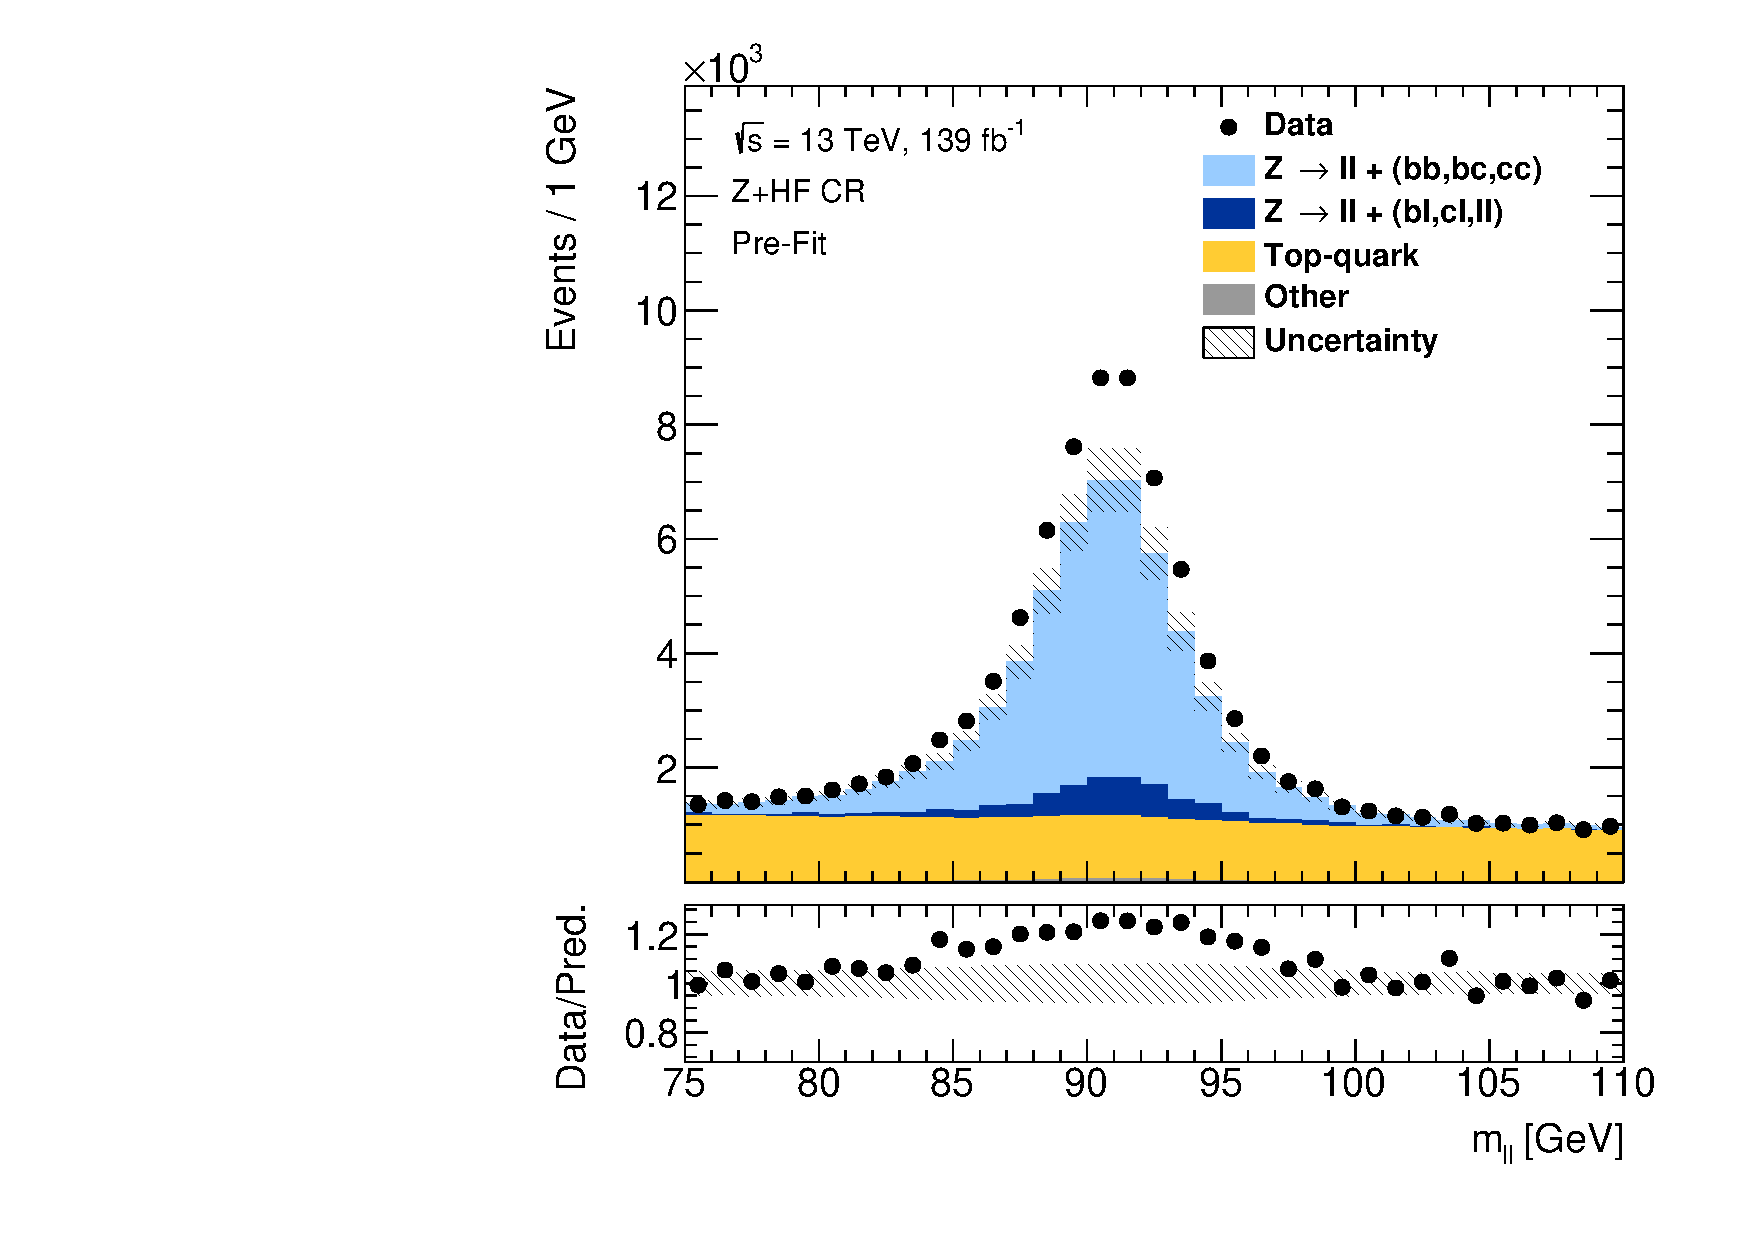
\includegraphics[width=0.55\textwidth]{zhfcr/Region_BMin0_incJet1_Y2015_DZllbbCR_T2_L2_distmLL_J2_Prefit_fixed}

  \caption{Distribution of the invariant di-lepton mass for the
    combination of electron- and muon-channel in the Z+HF control
    region prior to the likelihood fit. The contribution of \Zjets is
    sub-divided into cases where both $b$-jet candidates are matched
    to heavy flavour quarks ($b$ or $c$) and cases where at most one
    candidate is matched to heavy flavour quarks at generator-level.}
  \label{fig:zcr_mll_prefit}
\end{figure}



%%% Local Variables:
%%% mode: latex
%%% TeX-master: "../../phd_thesis"
%%% End:
